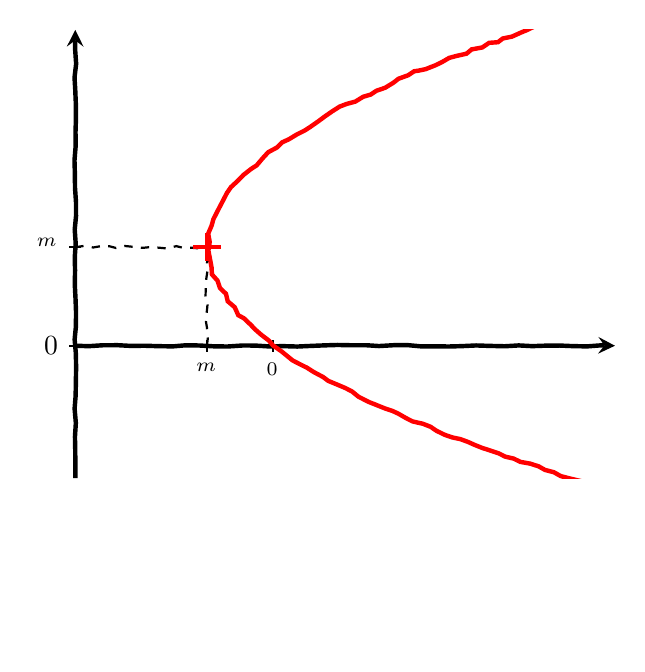
\begin{tikzpicture}%[decoration={random steps, segment length=1mm, amplitude=0.2pt}]
  \def\cxz{1.5}
  \def\KK{0.5}
  \def\czm{1.0}
  \def\cza{3.0}
  \def\cxm{1.0}
  \begin{axis}[%
      style = {ultra thick, black},
      axis x line = middle,
      axis y line = left,
      xlabel = {\cd},
      ylabel = {\cl},
      y label style = {at={(-0.05,0.95)},rotate=-90},
      xtick = {\cxm,\cxz},
      xticklabels = {$\Cd^m$,$\Cd^0$},
      ytick = {0,\czm},
      yticklabels = {0,$\Cl^m$},
      xmin = 0, xmax = 4.1,
      % ymax = 4.1,
      decoration={random steps,segment length=5pt,amplitude=0.3pt},%decorate,
      every tick/.style={thick,black,decorate}
    ]
    \begin{scope}[decoration={random steps,segment length=3pt,amplitude=0.5pt},decorate]
      \addplot[ultra thick,red,domain = -1:3,samples=30,samples y=0] ({\cxz+\KK*(\cza*x)*((\cza*x)-2*\czm)},{\cza*x});
      % \addplot[only marks] coordinates ({\cxm},{\czm});
      % \node[mark=+] (axis cs: \cxm,\czm){};
      \draw[dashed,thick, black, decorate] (axis cs: 0,\czm) -- (axis cs: \cxm,\czm);
      \draw[dashed,thick, black, decorate] (axis cs: \cxm,0) -- (axis cs: \cxm,\czm);
    \end{scope}
    \addplot [ultra thick, red, mark=+, mark size=5, mark options={solid}, only marks, forget plot]
    coordinates{(\cxm,\czm)};
  \end{axis}

\end{tikzpicture}